\documentclass[12pt,a4paper]{article} 

\usepackage{amsmath,amsfonts,amssymb,latexsym,graphicx,array}
\usepackage[french]{babel}
\usepackage[T1]{fontenc} 
\usepackage[utf8]{inputenc}
\usepackage{color}
\usepackage[a4paper, margin={3cm, 3cm}]{geometry}
\usepackage{subfigure}
\usepackage{epstopdf}



\begin{document}
%%%%%%%%%%%%%%%%%%%%%%%%%%%%%%%%%%%%%%%%%%%%%%%%%%%%%%%%%%%%%%%%%%%%%%%%%%%%%%%%%%%%%%%%%%%%%
% page titre
%%%%%%%%%%%%%%%%%%%%%%%%%%%%%%%%%%%%%%%%%%%%%%%%%%%%%%%%%%%%%%%%%%%%%%%%%%%%%%%%%%%%%%%%%%%%%
\setcounter{page}{0}


\begin{center}

% logo
\begin{minipage}[l]{.49\linewidth}
	\flushleft
\includegraphics[width=4cm]{img/logo_ENSTA.jpg}
\end{minipage}
\begin{minipage}[r]{.49\linewidth}
	\flushright
\includegraphics[width=4cm]{img/logo_CNAM.png}
\end{minipage}
\vspace{1.5cm}

% titre
\hrule \vspace{0.5cm}
\begin{LARGE}
	\textbf{FAT -- Projet Vélib}\\
\end{LARGE}
\vspace{0.5cm} \hrule
\vspace{3cm}

% noms
\definecolor{carmine}{rgb}{0.59, 0.0, 0.09}
\begin{Large}\color{carmine}
	Emmanuel JAY\\
	Adrien MAR\'ECHAL\\
	Benoît MULOCHER\\
\end{Large}
\vspace{5cm}

% Nom écoles
\begin{large}
	\textit{Conservatoire National des Arts et Métiers\\
	--\\
	\'Ecole Nationale Supérieure de Techniques Avancées\\}
\end{large}
\vfill

% date
\today
\end{center}

\thispagestyle{empty}
\newpage

%%%%%%%%%%%%%%%%%%%%%%%%%%%%%%%%%%%%%%%%%%%%%%%%%%%%%%%%%%%%%%%%%%%%%%%%%%%%%%%%%%%%%%%%%%%%%
%%%%%%%%%%%%%%%%%%%%%%%%%%%%%%%%%%%%%%%%%%%%%%%%%%%%%%%%%%%%%%%%%%%%%%%%%%%%%%%%%%%%%%%%%%%%%


\section{Définition du modèle}

\begin{figure}[h]
	\centering
	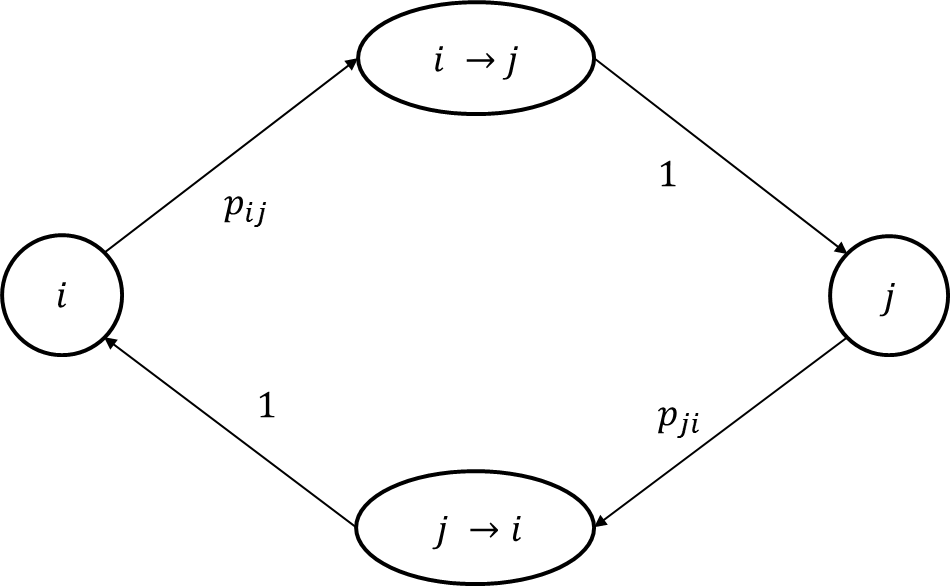
\includegraphics[width=0.6\linewidth]{img/modele.png}
	\caption{Schéma tout pourri du modèle de base, où on a représenté que 2 nœuds/stations et les trajets les reliant. Les valeurs sur les arcs indiquent les probabilités de transition.}
	\label{fig:1}
\end{figure}

On a des nœuds $i$ qui correspondent aux stations et des nœuds $i\rightarrow j$, notés $(ij)$, qui correspondent au trajets entre les stations, $i$ et $j$ décrivant l'ensemble des stations.\\

En reprenant les notations du papier "colony" :\\

On note $T_{a,b}(n)$ l'opérateur de transition, avec $(a,b) \in \left\{ \left(i,(ij)\right), i,j \in stations \right\} \cup \left\{ \left((ij),j\right), i,j \in stations \right\}$.\\


Transition rates :
\[
q\left(n, T_{a,b} (n) \right) = \lambda_{a,b} \phi_b(n_b)
\]

avec $\lambda_{a,b} = (proba\_transition\_a\_b) \times (temps\_service\_en\_a)$\\

On note $\lambda_a = \sum_b \lambda_{a,b}$ le paramètre du temps de service en $a$.

Lorsque $a = i$ est une stations, $\lambda_i$ correspond au taux de départ (horaire) de la station. Lorsque l'on considère un trajet $a = (ij)$, $\lambda_{(ij)})$ correspond au temps de trajet entre $i$ et $j$.\\


En notant $p_{ij}$ la probabilité d'emprunter le chemin vers $j$ depuis la stations $i$ (i.e. la proba de la transition $\left(i,(ij) \right)$), on a
\[
\lambda_{i,(ij)} = p_{ij} \lambda_i
\]

D'autre part, comme on a des proba de transition de $1$ depuis un chemin vers sa destination, on a
\[
\lambda_{(ij),j} = \lambda_{(ij)}
\]


\section{Matrice de routage}




\section{\'Equations de trafic}

En reprenant les notations du papier "colony" :\\

L'équation $(2.1)$ du papier, après avoir fait apparaître les probabilités de transition, devient pour notre problème
\begin{equation}
\alpha_{(ij)} \lambda_{(ij)} = \alpha_i p_{ij} \lambda_i
\label{eq:trafic_1}
\end{equation}
pour une transition à travers un chemin $(ij)$, et
\begin{equation}
\alpha_j \sum_k p_{jk} \lambda_j = \sum_k \alpha_{(kj)} \lambda_{(kj)}
\label{eq:trafic_2}
\end{equation}
pour une transition par une stations $j$.

Comme $\sum_k p_{jk} = 1$, on a donc
\begin{equation}
\alpha_j \lambda_j = \sum_k \alpha_{(kj)} \lambda_{(kj)}
\label{eq:trafic_2_bis}
\end{equation}
pour la transition par la station $j$.\\

En injectant l'expression des $\alpha_{(ij)}$, on obtient
\begin{equation}
\alpha_j = \frac{1}{\lambda_j} \sum_i \alpha_i p_{ij} \lambda_i
\end{equation}


Par ailleurs, on a les conditions
\[
\alpha_i > 0, \quad \alpha_{(ij)} >0, \quad \forall i,j \in stations 
\]
et
\begin{equation}
\sum_i \alpha_i + \sum_i \sum_j \alpha_{(ij)} = 1
\end{equation}
i.e.
\begin{equation}
\sum_i \left(1 + \lambda_i \sum_j \frac{p_{ij}}{\lambda_{(ij)}} \right) \alpha_i = 1
\end{equation}

~\\
Pour résoudre cette crotte, il suffit de résoudre
\begin{equation}
\alpha = \alpha P
\end{equation}
où $\alpha$ est le vecteur ligne des $\alpha_i, i \in stations$. Et $P$ est la matrice dont les coefficients sont donnés par $\left( p_{ij} \frac{\lambda_i}{\lambda_j} \right)_{i,j \in stations}$.\\

Pour ce faire, il suffit d'inverser la matrice $(I-P)$ dans laquelle on a remplacé une colonne par le vecteur formés par $\left(1 + \lambda_i \sum_j \frac{p_{ij}}{\lambda_{(ij)}} \right)_{i \in stations}$, et on utilisant un second membre nul, sauf pour la colonne correspondant à celle modifiée qui doit comporter un $1$.
 
On calculera ainsi les $\alpha_i$, d'où découlerons ensuite les $\alpha_{(ij)}$ (si tant est qu'ils nous intéressent) grâce à l'équation (\ref{eq:trafic_1}).



\section{Remarques}

C'est peut être du gros caca.

Quoi qu'il en soit, dans le premier jeu de données qu'il a fournit, il n'y rien qui nous permette de calculer les temps de service (i.e. les temps de trajets pour les nœuds de trajet et le taux horaire de départ pour les nœuds de station). Il donne néanmoins ces temps dans le deuxième jeu de données, où j'avais vu un exemple de matrice de routage. C'est donc bien que ça doit servir.

Il serait étonnant que les équations de trafic ne fassent pas intervenir les temps de service, donc même dans le cas où ce que j'ai fait ici est incorrect, on est coincé pour la résolution.



\end{document}